\documentclass{standalone}

\usepackage{tikz}
\usepackage{standalone}
\usetikzlibrary{arrows}
\usetikzlibrary{decorations.markings}
\usetikzlibrary{calc}

\begin{document}
    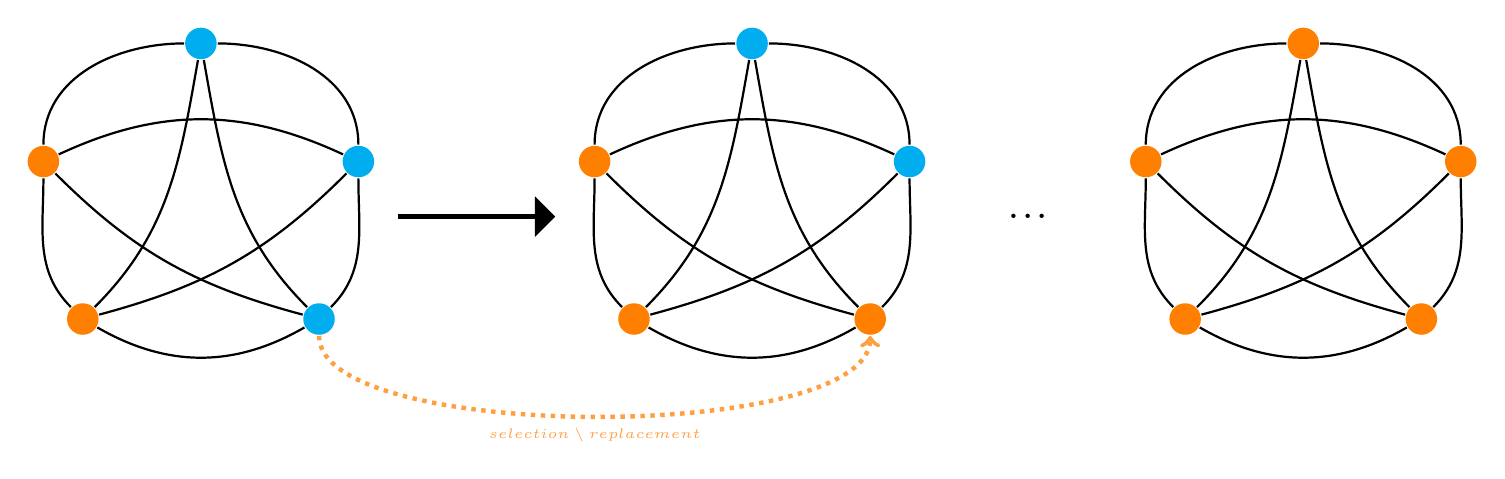
\begin{tikzpicture}

    \tikzstyle{state}=[minimum width=0.4cm, font=\boldmath];

    % , label=above:{\small{\textit{starting population}}}]
    \node[circle, fill=cyan, thick] (0) at (0, 1.5) [state]   {};
    \node[circle, fill=orange, thick] (1) at (-2, 0) [state]  {};
    \node[circle, fill=orange, thick] (2) at (-1.5, -2) [state] {};
    \node[circle, fill=cyan, thick, thick] (3) at (1.5, -2) [state]  {};

    \node[circle, fill=cyan, thick] (4) at (2, 0) [state]   {};

    \draw[ultra thick, -triangle 90] (2.5, -0.7) -- (4.5, -0.7);

    \draw (0) edge[out=180, in=90, -, thick] node [above] {} (1);
    \draw (0) edge[out=0, in=90, -, thick] node [above] {} (4);
    \draw (1) edge[out=-90, in=135, -, thick] node [above] {} (2);
    \draw (2) edge[out=-30, in=-150, -, thick] node [above] {} (3);
    \draw (4) edge[out=-90, in=45, -, thick] node [above] {} (3);

    \draw (2) edge[out=15, in=-135, -, thick] node [above] {} (4);
    \draw (3) edge[out=165, in=-45, -, thick] node [above] {} (1);

    \draw (0) edge[out=-100, in=45, -, thick] node [above] {} (2);
    \draw (0) edge[out=-80, in=135, -, thick] node [above] {} (3);

    \draw (1) edge[out=25, in=155, -, thick] node [above] {} (4);

    % , label=above:{\small{\textit{birth - death stage}}}]
    \node[circle, fill=cyan, thick] (5) at (7, 1.5) [state]   {};
    \node[circle, fill=orange, thick] (6) at (5, 0) [state]  {};
    \node[circle, fill=orange, thick] (7) at (5.5, -2) [state] {};
    \node[circle, fill=orange, thick] (8) at (8.5, -2) [state]  {};
    \node[circle, fill=cyan, thick] (9) at (9, 0) [state]   {};

    \draw (3) edge[out=-90, in=-90, ->, ultra thick, orange!75, dotted, looseness=0.5] node [below] {\tiny{\textit{$selection \setminus replacement$}}} (8);

    \draw (5) edge[out=180, in=90, -, thick] node [above] {} (6);
    \draw (5) edge[out=0, in=90, -, thick] node [above] {} (9);
    \draw (6) edge[out=-90, in=135, -, thick] node [above] {} (7);
    \draw (7) edge[out=-30, in=-150, -, thick] node [above] {} (8);
    \draw (9) edge[out=-90, in=45, -, thick] node [above] {} (8);

    \draw (7) edge[out=15, in=-135, -, thick] node [above] {} (9);
    \draw (8) edge[out=165, in=-45, -, thick] node [above] {} (6);

    \draw (5) edge[out=-100, in=45, -, thick] node [above] {} (7);
    \draw (5) edge[out=-80, in=135, -, thick] node [above] {} (8);

    \draw (6) edge[out=25, in=155, -, thick] node [above] {} (9);

    \node (s) at (10.5, -0.7) [state]   {$\dots$};

    % , label=above:{\small{\textit{stable opulation}}}]
    \node[circle, fill=orange, thick] (10) at (14, 1.5) [state]   {};
    \node[circle, fill=orange, thick] (11) at (12, 0) [state]  {};
    \node[circle, fill=orange, thick] (12) at (12.5, -2) [state] {};
    \node[circle, fill=orange, thick] (13) at (15.5, -2) [state]  {};
    \node[circle, fill=orange, thick] (14) at (16, 0) [state]   {};

    \draw (10) edge[out=180, in=90, -, thick] node [above] {} (11);
    \draw (10) edge[out=0, in=90, -, thick] node [above] {} (14);
    \draw (11) edge[out=-90, in=135, -, thick] node [above] {} (12);
    \draw (12) edge[out=-30, in=-150, -, thick] node [above] {} (13);
    \draw (14) edge[out=-90, in=45, -, thick] node [above] {} (13);

    \draw (12) edge[out=15, in=-135, -, thick] node [above] {} (14);
    \draw (13) edge[out=165, in=-45, -, thick] node [above] {} (11);

    \draw (10) edge[out=-100, in=45, -, thick] node [above] {} (12);
    \draw (10) edge[out=-80, in=135, -, thick] node [above] {} (13);

    \draw (11) edge[out=25, in=155, -, thick] node [above] {} (14);
\end{tikzpicture}

\end{document}